\chapter{CPU-Net Result}\label{chap:cpu-net_result}

\section{Introduction}

Neutrinoless double-beta decay is primarily a single sited events. Low-background HPGe experiments such as LEGEND thus seeks to distinguish between single site from multi site events. The FEP peak is an excellent region for training given its abundance and the fact that it contains a mixture of single and multi-site events. SEP and DEP can then be used as a validation data set, evaluating the model's response to multi-site and single-site events, respectively.


\section{Training progression}
The progression of training losses is shown in Fig. \ref{fig:training_loss}. The cycle-consistent and identity losses converge rapidly towards zero, indicating that the model effectively learns waveform features while preserving both identity and cycle consistency. Additionally, the adversarial interaction between the generator and discriminators is evident. Early in training, the discriminator initially “wins,” causing its loss to decrease and the generator’s loss to increase. As training continues, the generator improves, and both networks approach an equilibrium in which each attempts to outcompete the other. In this state, both loss functions fluctuate as they continuously adapt and improve.


\begin{figure}%[htb!]
    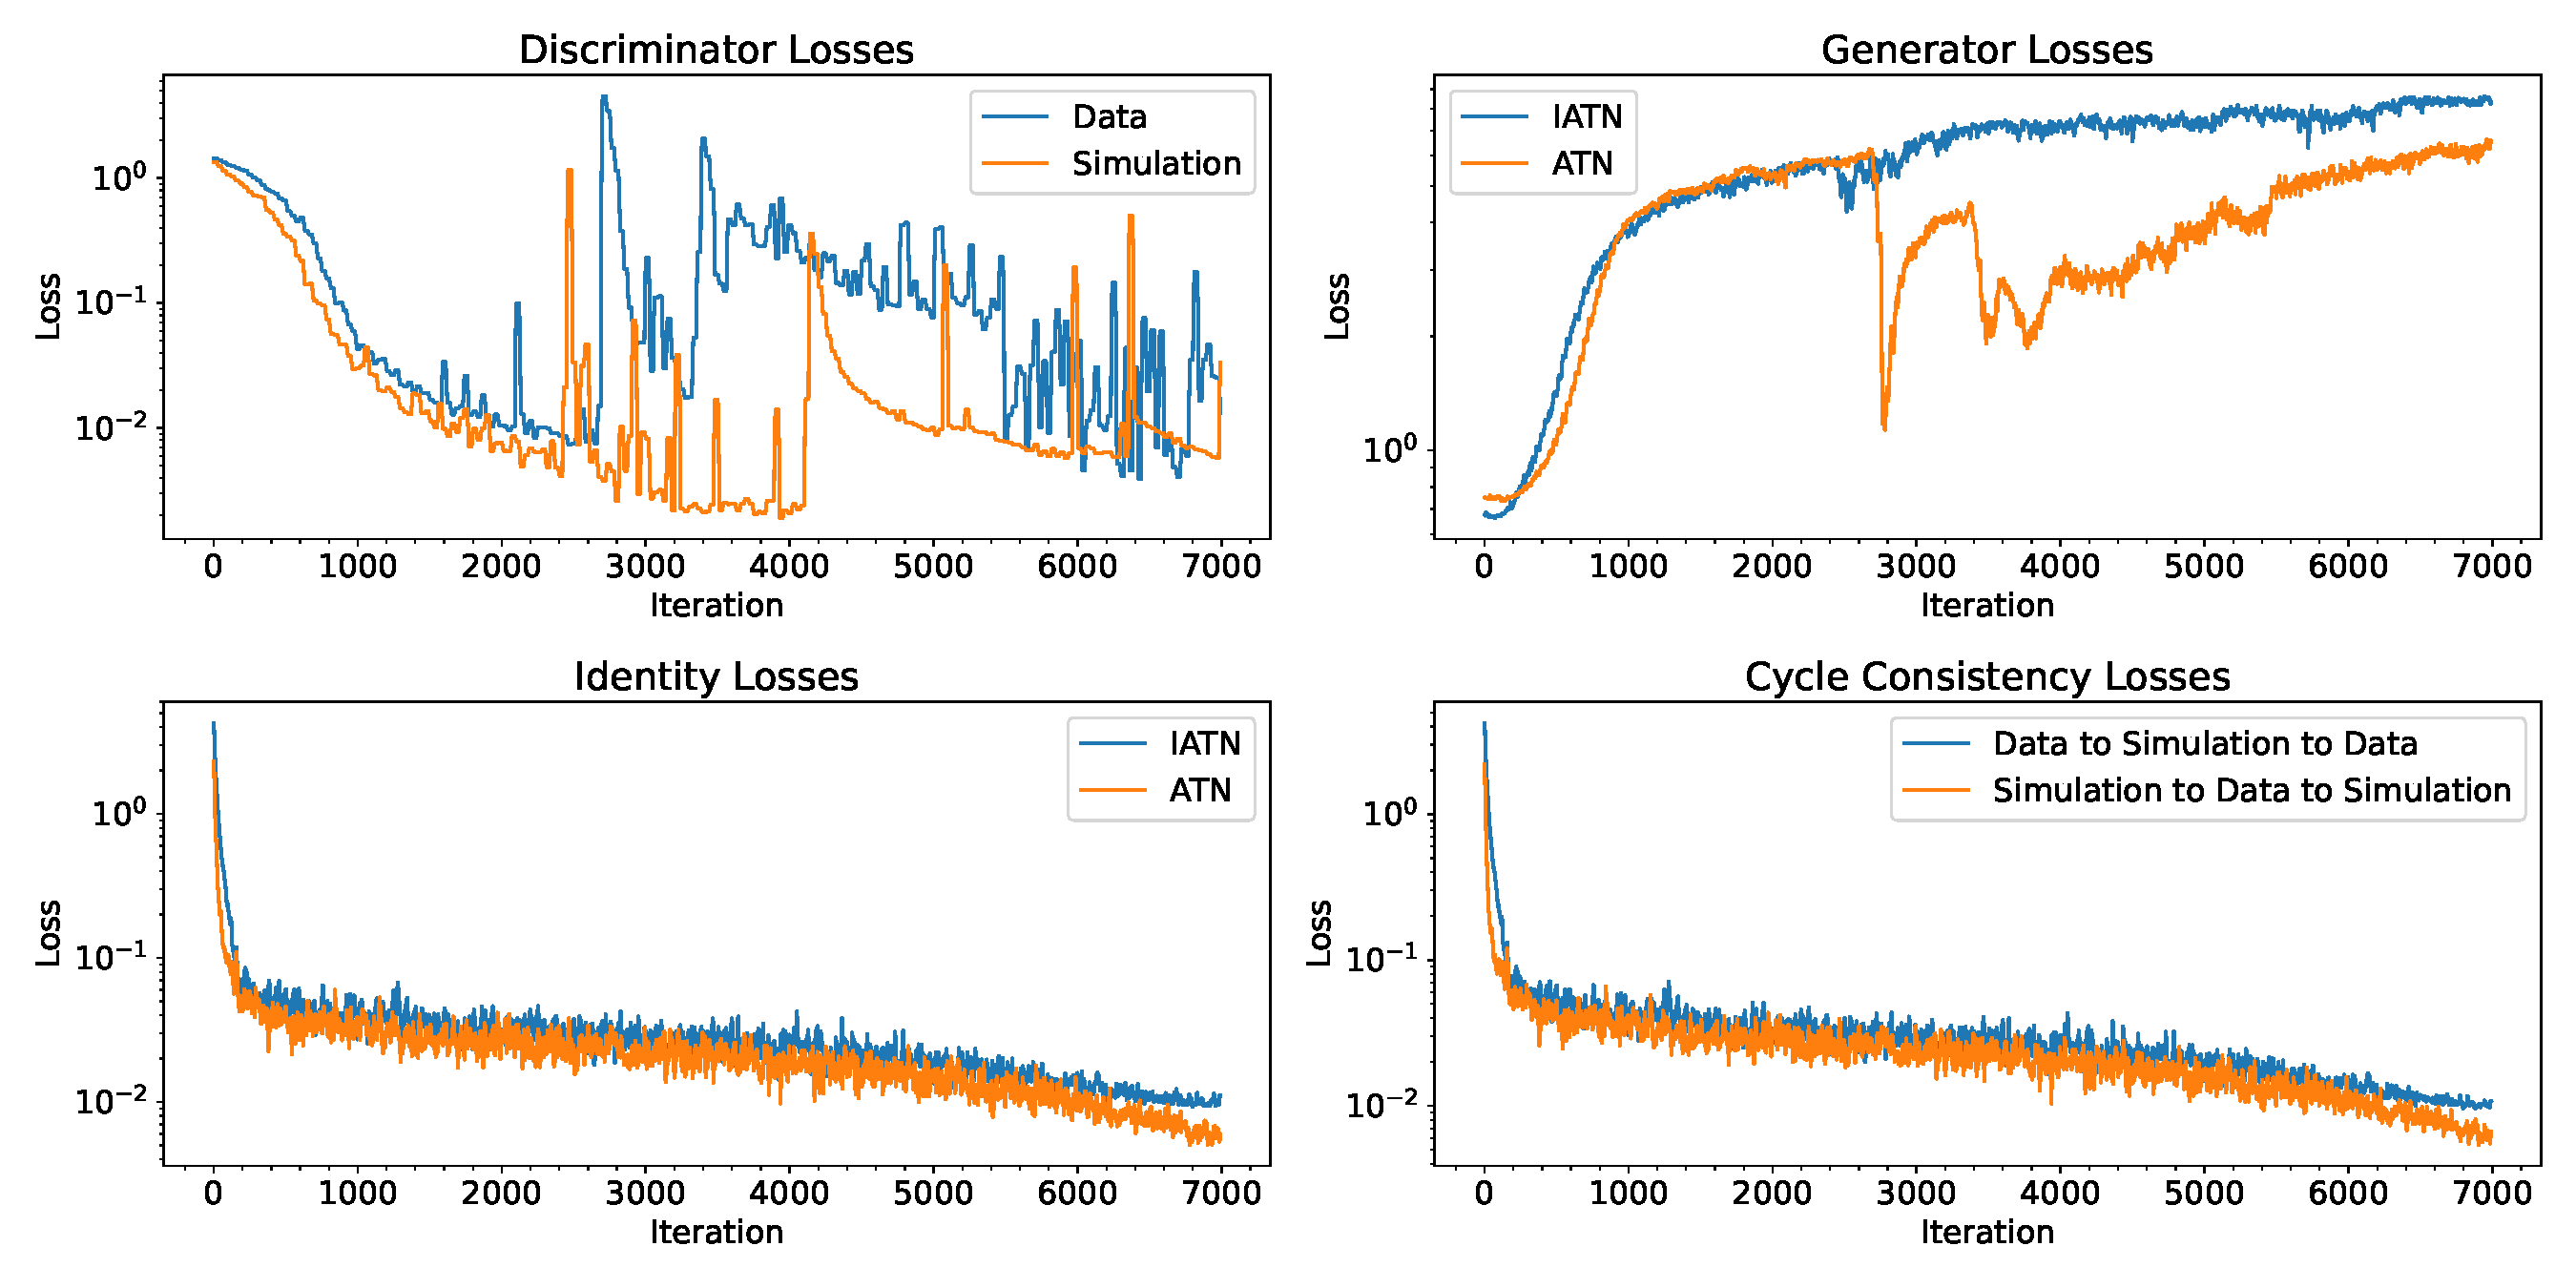
\includegraphics[width=0.99\linewidth]{ch8/figs/loss_funcs.pdf}
    \caption{Training losses for CPU-Net. Losses have been smoothed using a moving average of 10 samples for clarity. The identity and Cycle losses rapidly converged to zero while the generator and discriminator losses fluctuate.} 
   \label{fig:training_loss}
\end{figure}

 % The translation of simulated waveform is shown in Fig \ref{fig:current_amp}. The ATN translates the simulated waveform to the ATN output by smoothing the sharp turning edge in the grey region. This is a consequence of the non-zero integration time in detector waveforms, which is set to $0$ in \texttt{siggen}. The RC discharge effect of the electronic readout system is also set to 0 in \texttt{siggen}, leading to a tail slope of 0 in the simulated waveforms. The ATN learns to translate the flat tail in the cyan region into an exponential decay, and the strength of the decay can be measured by the tail slope reconstruction parameter $c_{tail}$.

% \begin{figure}[htb!]
%     \includegraphics[width=0.99\linewidth]{ch8/figs/ATN.png}
%     \caption{An example ATN output (blue) generated by the input simulated waveform (red). A detector waveform (dotted magenta,randomly drawn from data) is also illustrated as a reference. The grey region depicts the area where the preamplifier integration effect is most visible. The blue region shows the impact of the RC circuit discharge effect.} 
%    \label{fig:sample_result}
% \end{figure}

\section{Waveform Translation}
To validate the model’s performance, we applied CPU-Net to waveforms at the single-escape peak (SEP) and double-escape peak (DEP) energies, which test the model’s accuracy on multi-site (SEP) and single-site (DEP) events, respectively. Over $90\%$ of SEP events are multi-site, and over $90\%$ DEP events are single site. Fig. \ref{fig:cycle_bab} and \ref{fig:cycle_aba}  shows the cycle consistency in the CPU-Net on SEP waveforms. The network effectively translates the waveforms in forward and reverse translations. The data waveform tail has a downward slope that is a result of the long exponential resistor-capacitor (RC) decay of the preamplifier output waveform. In the \texttt{siggen} simulations, the RC discharge effect is not modeled, resulting in a flat tail slope of zero. ATN learns to transform this flat tail into an exponentially decaying one, matching the observed behavior in real detector data, and IATN learns to transform it back to zero slope matching the simulations.

% A simple way to understand the electronics response is to look at the signal waveform tail. . This is usually corrected in post signal processing stage where the `pole' cause by the RC decay is corrected by integrating a `zero' into the transfer functions, called pole-zero correction. While the pole-zero correction has proved reliable for HPGe experiments, it is a first order correction and often higher corrections are warranted. \cite{MJD_electronics}\cite{mjd_pole_zero}

\begin{figure}%[htb!]
    \centering
    %trim={0pc 0pc 0pc 3pc},clip
    \includegraphics[width=0.99\linewidth]{ch8/figs/SEP_result_comp_1x3_cycle_BAB.pdf}
    \caption{Illustration of bi-directional cycle consistency in waveform translation. Starting with 10 simulated waveforms, the ATN first translates them into detector-like waveforms, and the IATN then returns them to the simulated domain.}
    \label{fig:cycle_bab}
\end{figure}

\begin{figure}%[htb!]
    \centering
    %trim={0pc 0pc 0pc 3pc},clip
    \includegraphics[width=0.99\linewidth]{ch8/figs/SEP_result_comp_1x3_cycle_ABA.pdf}
    \caption{Illustration of bi-directional cycle consistency in waveform translation. Beginning with 10 detector waveforms, the IATN translates them into simulated-like waveforms, and the ATN subsequently restores them to detector-like waveforms.}
    \label{fig:cycle_aba}
\end{figure}

\section{Validation on key waveform parameters}
\subsection{Drift Time Distribution}
\begin{figure}[htb!]
    \centering
    %trim={0pc 0pc 0pc 3pc},clip
    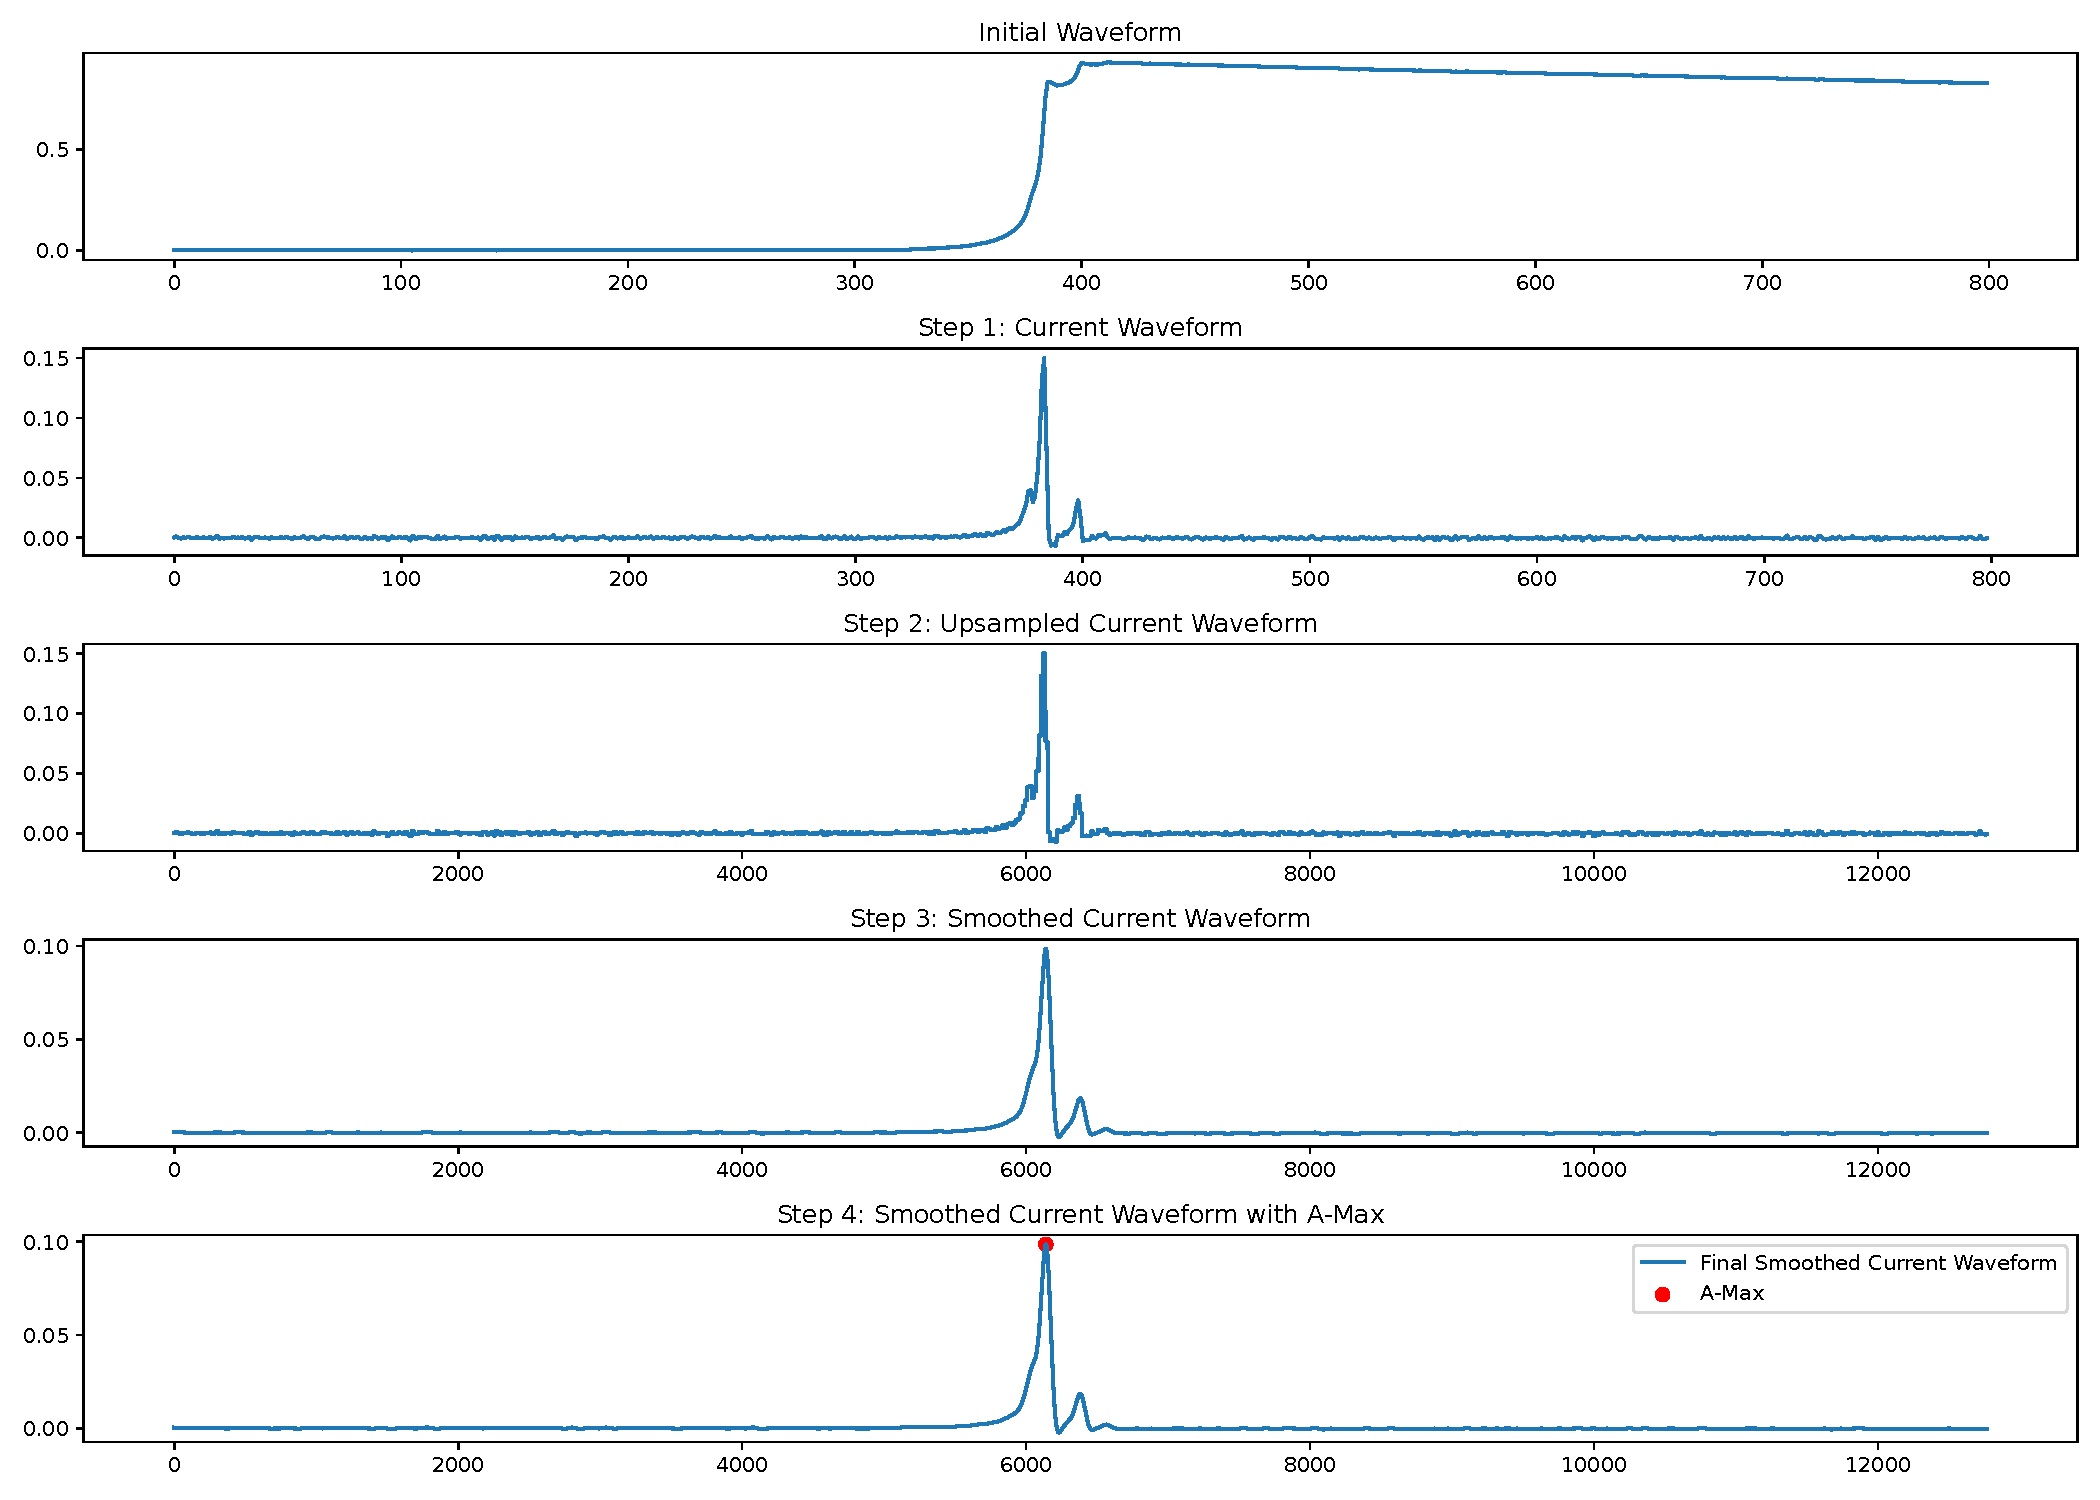
\includegraphics[width=0.99\linewidth]{ch8/figs/curr_amp_calc.pdf}
    \caption{Steps involved in calculating the maximum current amplitude of the waveform}
    \label{fig:ch8:curr_amp_calc}
\end{figure}

\begin{figure}[htb!]
    \centering
    %trim={0pc 0pc 0pc 3pc},clip
    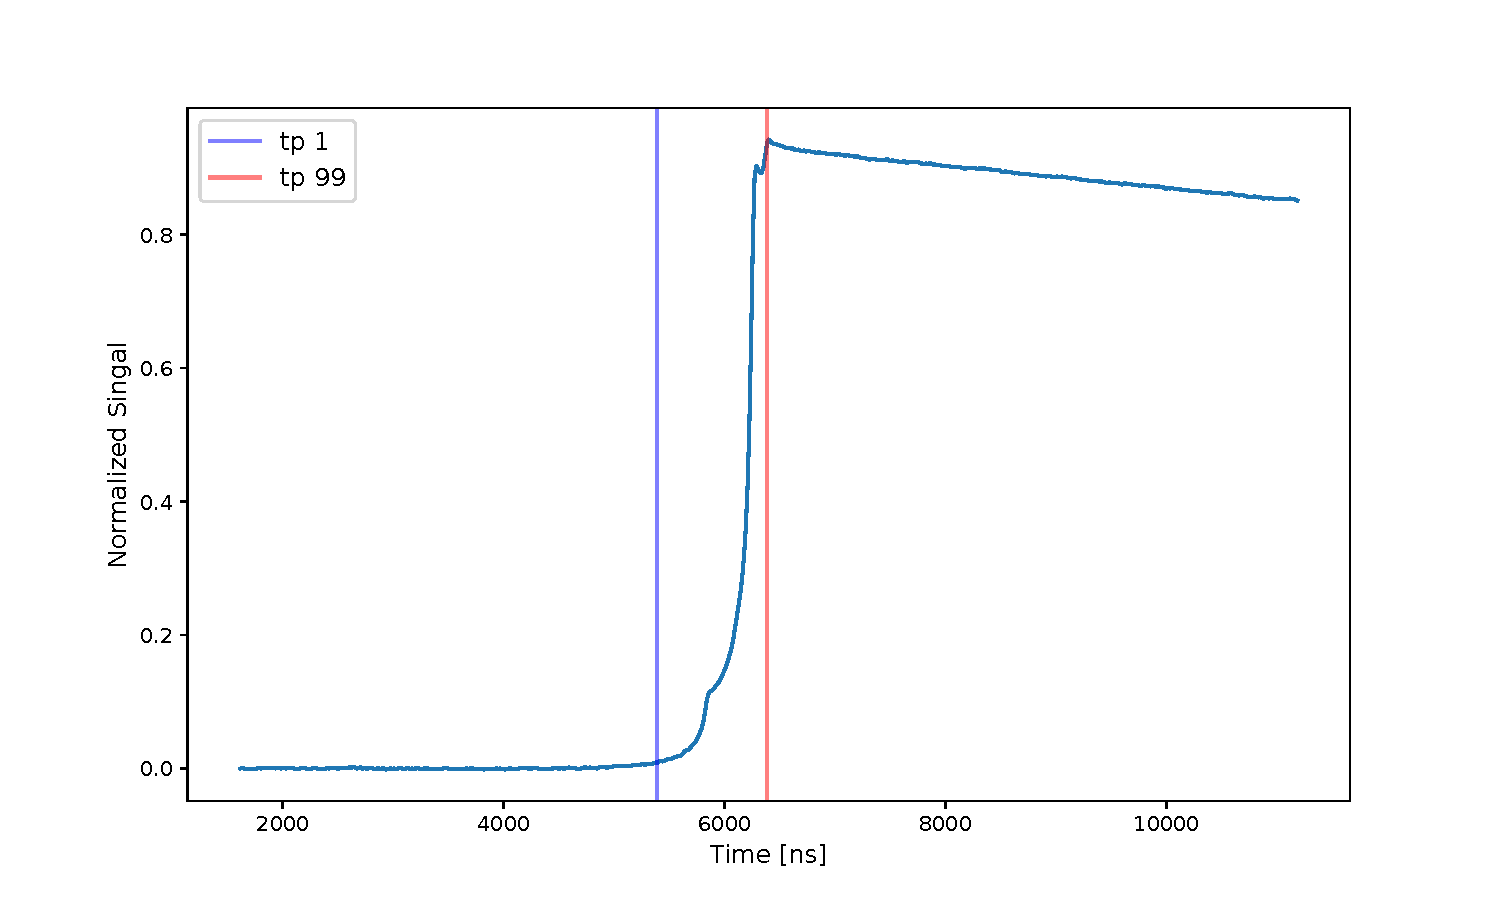
\includegraphics[width=0.99\linewidth]{ch8/figs/time_calc.pdf}
    \caption{Calculating the time points of the waveform}
    \label{fig:ch8:time_calc}
\end{figure}


 The accuracy of translations can be examined on a distribution level by plotting the histogram with respect to key reconstruction parameters. Figure \ref{fig:drift_times_sep} and \ref{fig:drift_times_dep} shows the distribution of drift time $T_{Drift}$. Data has a slower $T_{Drift}$ due to the effect of the preamp. ATN nets learn to slow the drift time of the waveforms while keeping matching the distribution of the data. We use the Intersection over Union (IoU) metric for measuring the overlap between distributions. The SEP $T_{Drift}$ IoU increases to $62.4\%$ from $39.5\%$.
 
\begin{figure}[htb!]
%[trim={left bottom right top},clip]
\centering
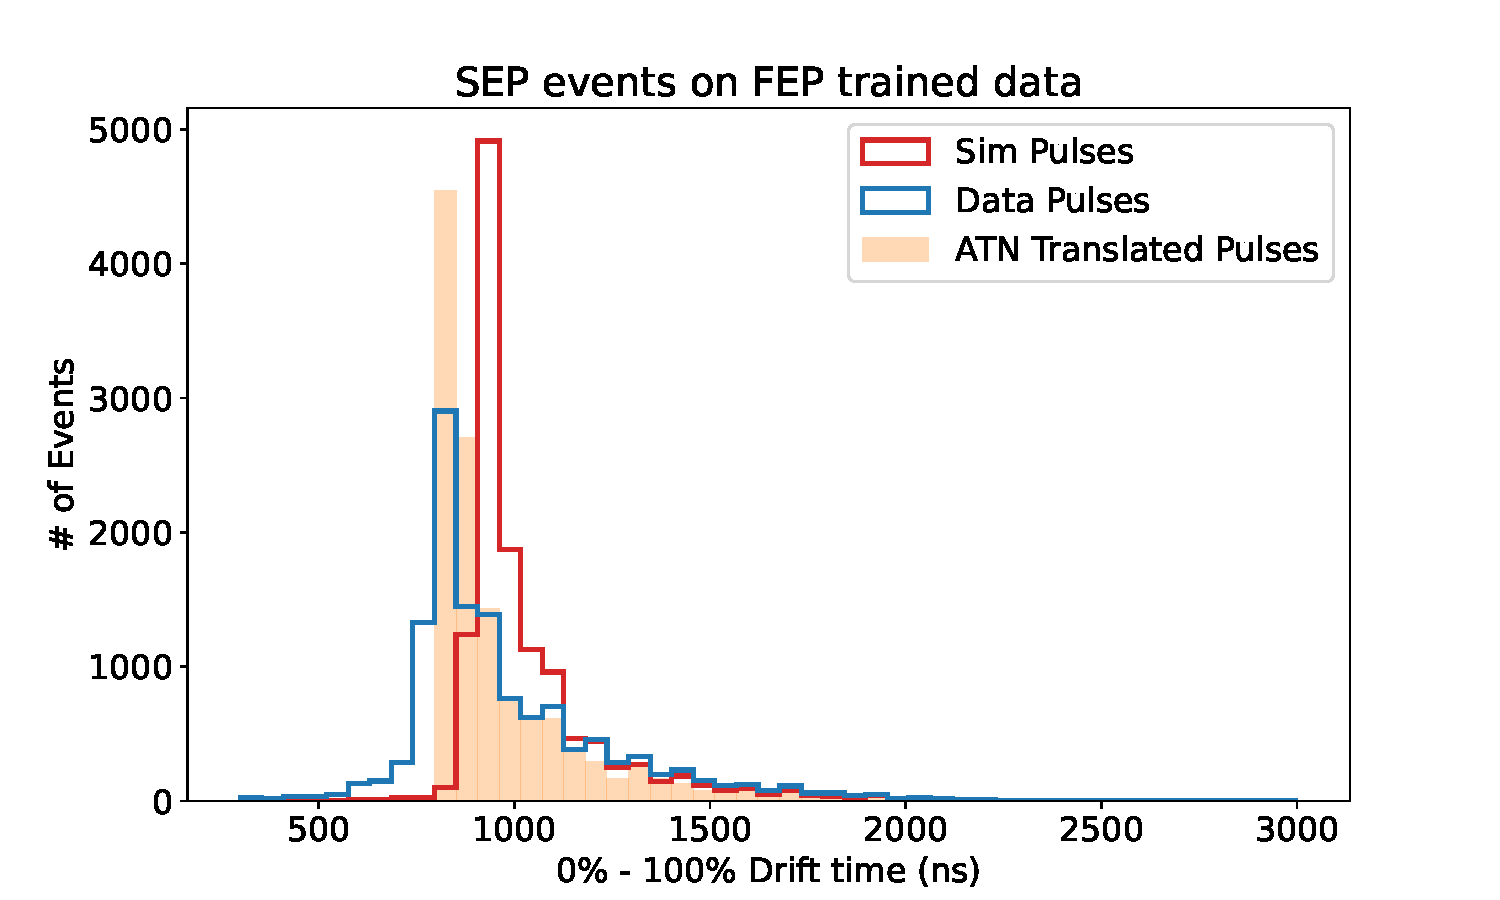
\includegraphics[width=0.99\linewidth,trim={0pc 0pc 0pc 0pc},clip]{ch8/figs/sep_drift_time.pdf}
\caption{The distribution of the 1\%–100\% drift time on SEP dataset.}
\label{fig:drift_times_sep}
\end{figure}

\begin{figure}[htb!]
%[trim={left bottom right top},clip]
\centering
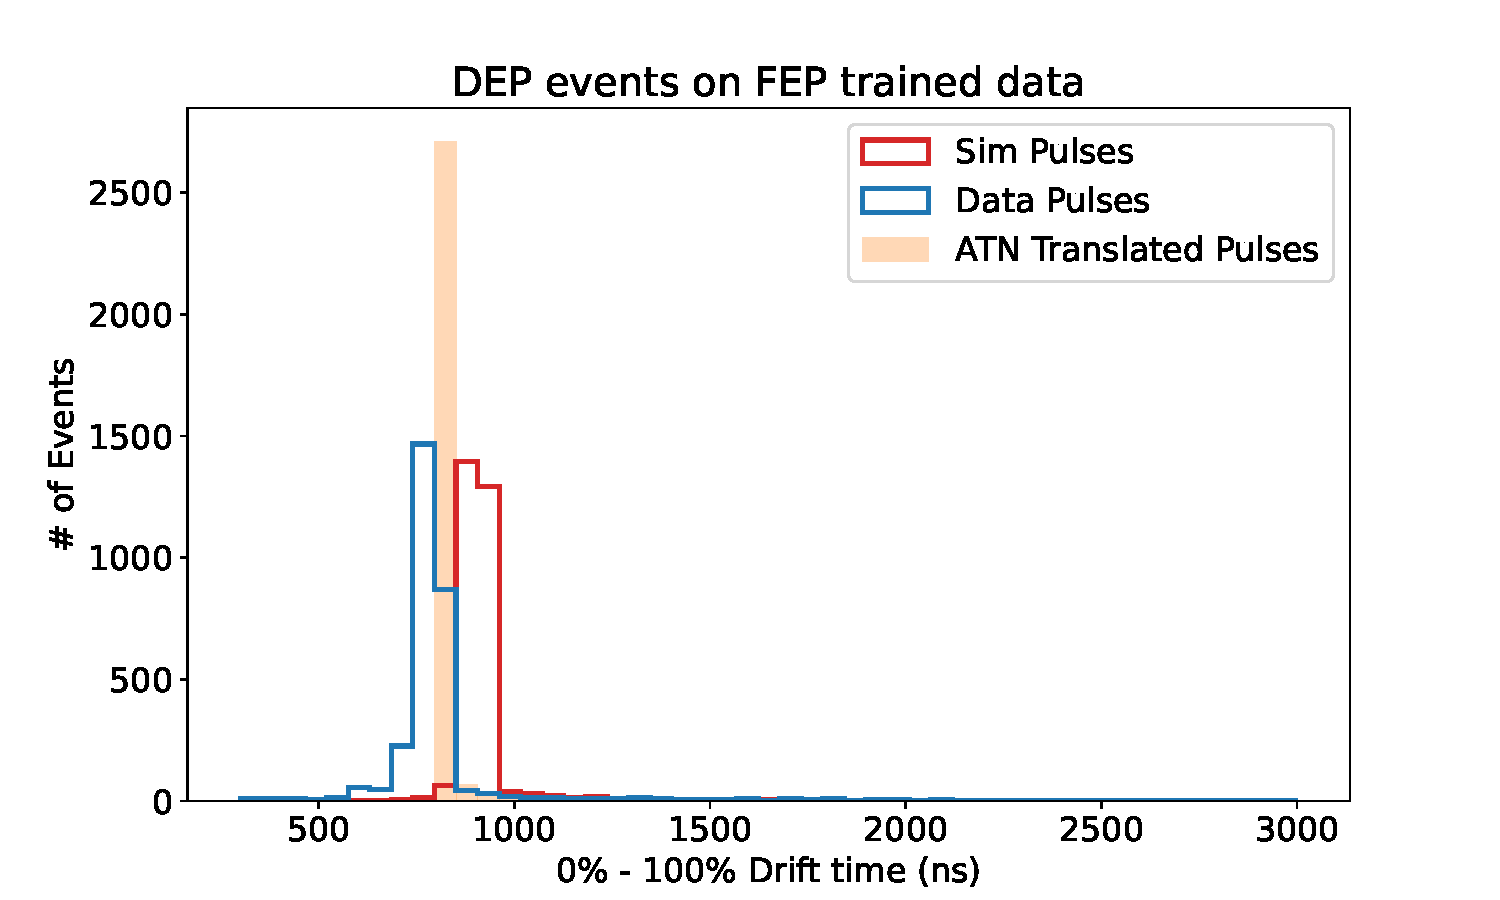
\includegraphics[width=0.95\linewidth,trim={0pc 0pc 0pc 0pc},clip]{ch8/figs/dep_drift_time.pdf}
\caption{The distribution of the 1\%–100\% drift time on DEP dataset.}
\label{fig:drift_times_dep}
\end{figure}

\subsection{Current Amplitude}

The maximum current amplitude ($I_{max}$) is determined by differentiating the waveform and identifying the maximum value of its derivative. For a given event energy, single-site events produce a localized energy deposition that leads to a sharper and faster-rising $I_{max}$, while multi-site events, with energy deposited at multiple locations within the detector, yield broader, slower-rising current peaks. This makes $I_{max}$ highly effective at distinguishing single-site from multi-site events and thus a crucial parameter in waveform shape simulations \cite{mjd_psd}. Figure \ref{fig:current_amp} shows the distribution of $I_{max}$.  ATN learns to correctly slow down the current amplitude of simulated waveforms to one that aligns with data. The SEP $I_{max}$ increases to IoU to $63.71\%$ from $27.53\%$.
  
\begin{figure}[htb!]
\centering
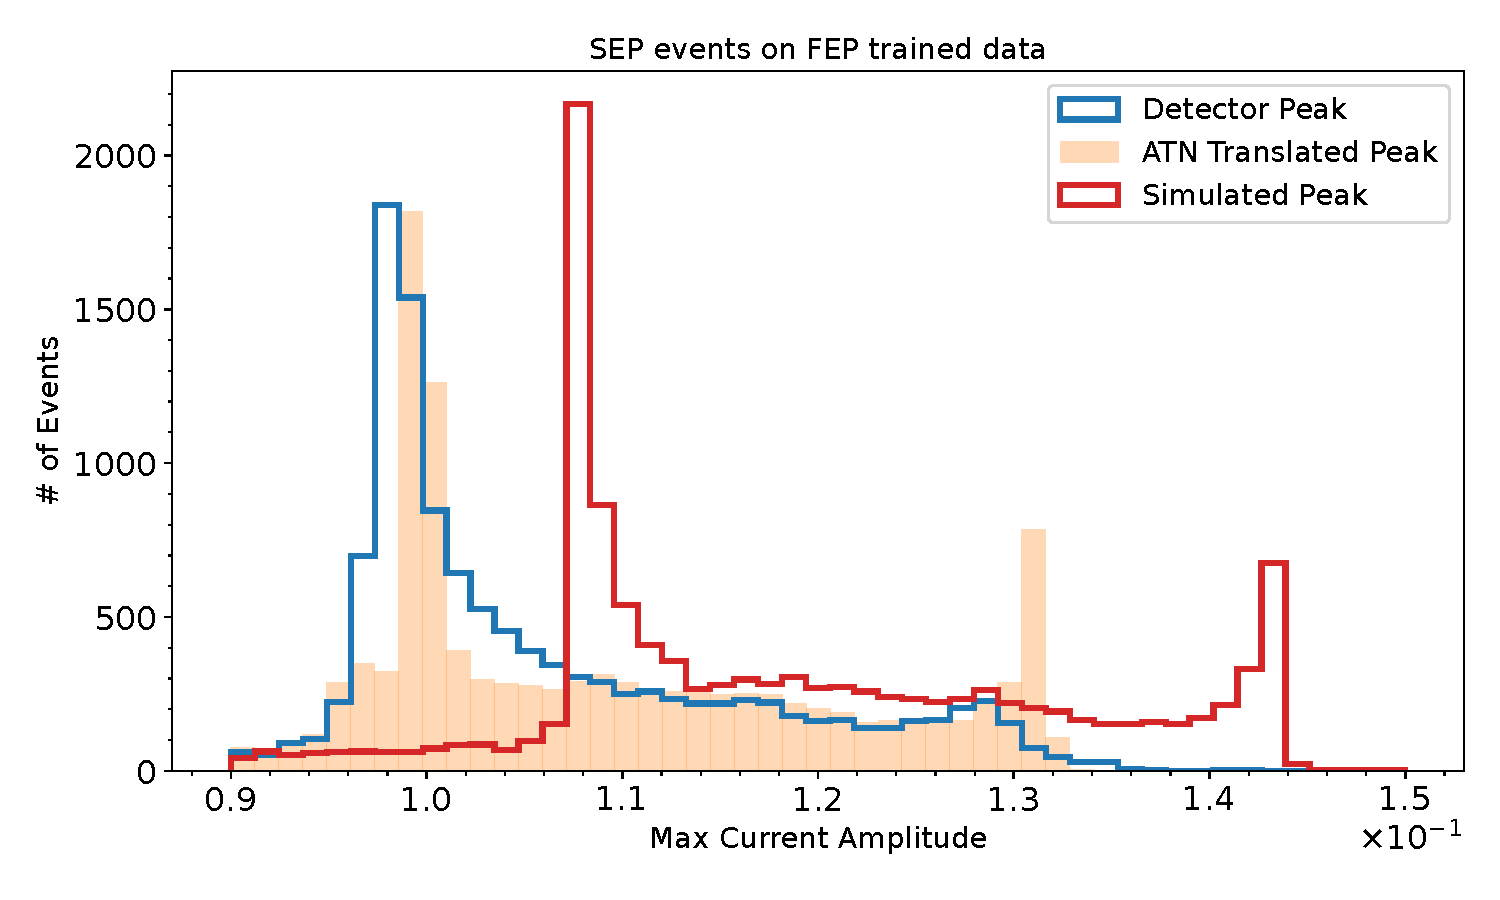
\includegraphics[width=0.99\linewidth,trim={0pc 0pc 0pc 0pc},clip]{ch8/figs/SEP_amp.pdf}
\caption{ Distribution of maximum current amplitude ($I_{max}$) on SEP validation datasets.}
\label{fig:current_amp_sep}
\end{figure}

\begin{figure}[htb!]
\centering
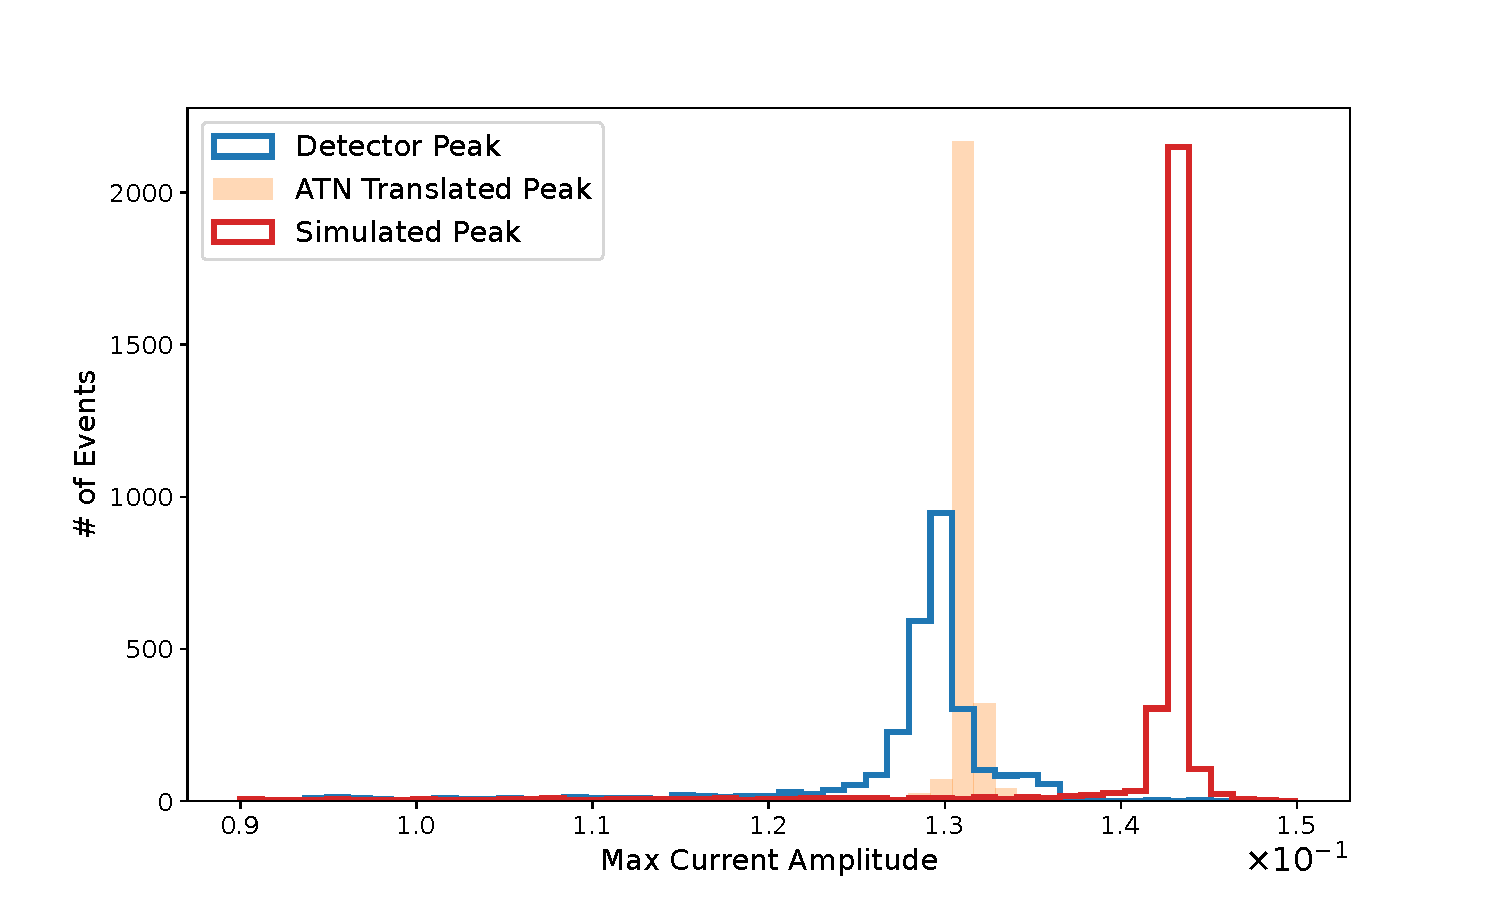
\includegraphics[width=0.99\linewidth,trim={0pc 0pc 0pc 0pc},clip]{ch8/figs/DEP_amp.pdf}
\caption{ Distribution of maximum current amplitude ($I_{max}$) on DEP validation datasets.}
\label{fig:current_amp_dep}
\end{figure}

The scatter plot between $I_{max}$ of simulated waveforms and ATN translated waveforms shows that ATN performs does this while mainting the relative order of events.

\begin{figure}[htb!]
\centering
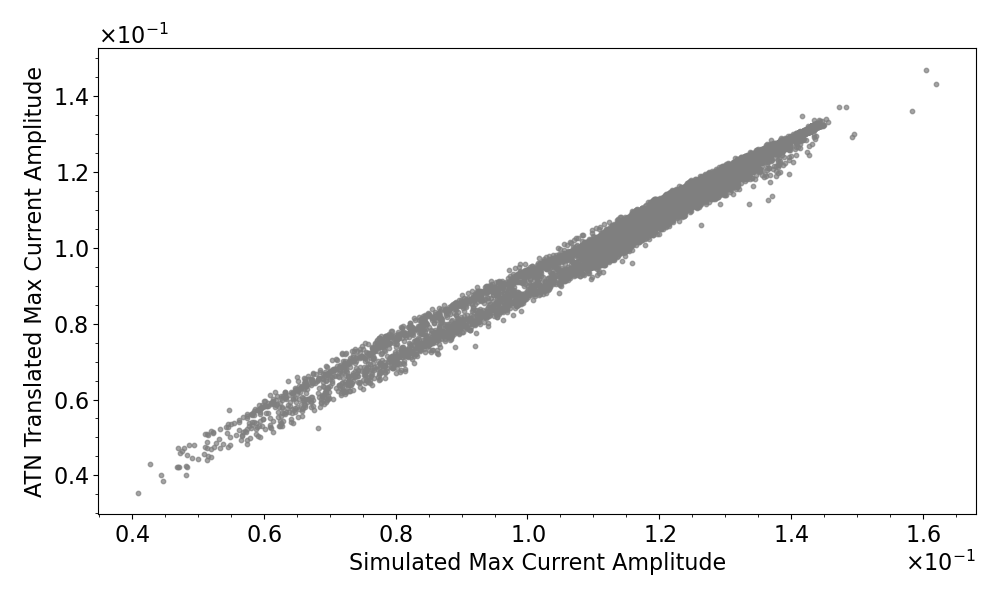
\includegraphics[width=0.99\linewidth,trim={0pc 0pc 0pc 0pc},clip]{ch8/figs/SEP_scatter_current_amplitude.png}
\caption{Scatter plot between $I_{max}$ of simulated waveforms and ATN translated waveforms. ATN shits the amplitude distribution to align with data while maintaining the relative ordering of individual events.}
\label{fig:current_amp}
\end{figure}



\subsection{Tail Slope}
The strength of the RC decay can be measured by the mean tail slope parameter $c_{tail}$. Simulated waveforms do not have a RC decay and thus have mean tail slope of zero, the data waveform were found to have tail slope of $-2.946\times10^{-4}$. The mean tail slop of ATN reconstructed waveform was found to be $-2.963\times10^{-4}$ for data like waveform, within $0.58\%$ of the actual value.

\begin{figure}[htb!]
\centering
%[trim={left bottom right top},clip]
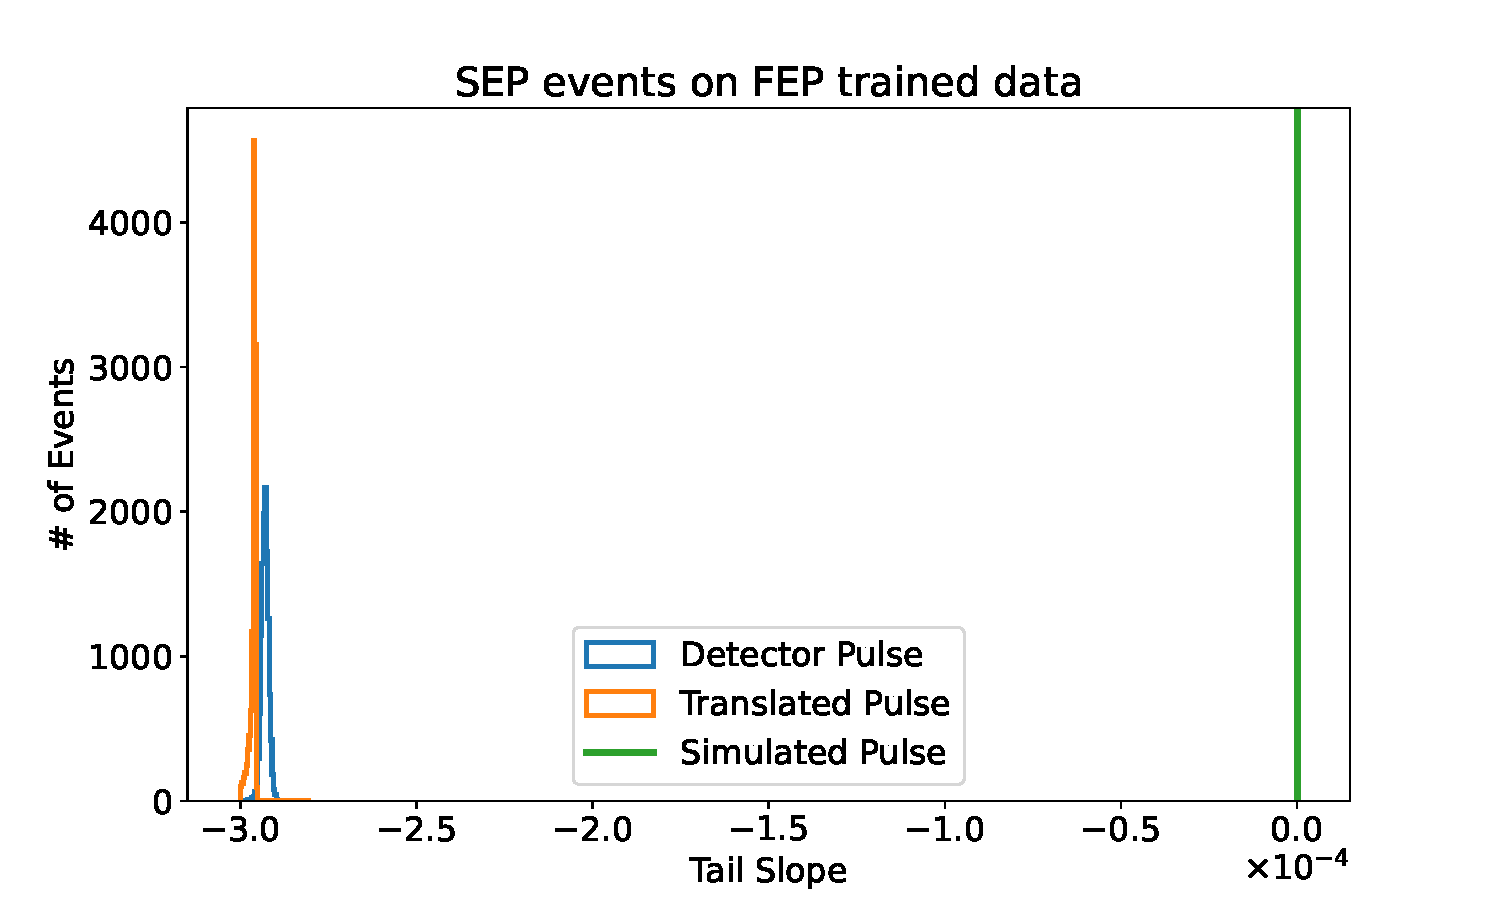
\includegraphics[width=0.97\linewidth,trim={2pc 0pc 2pc 0pc},clip]{ch8/figs/SEP_sim_ts.pdf}
\caption{ Distribution of Tail slope between data and ATN translated waveforms}
\label{ch8:fig:tail_slope_comp}
\end{figure}


\begin{figure}[htb!]
\centering
%[trim={left bottom right top},clip]
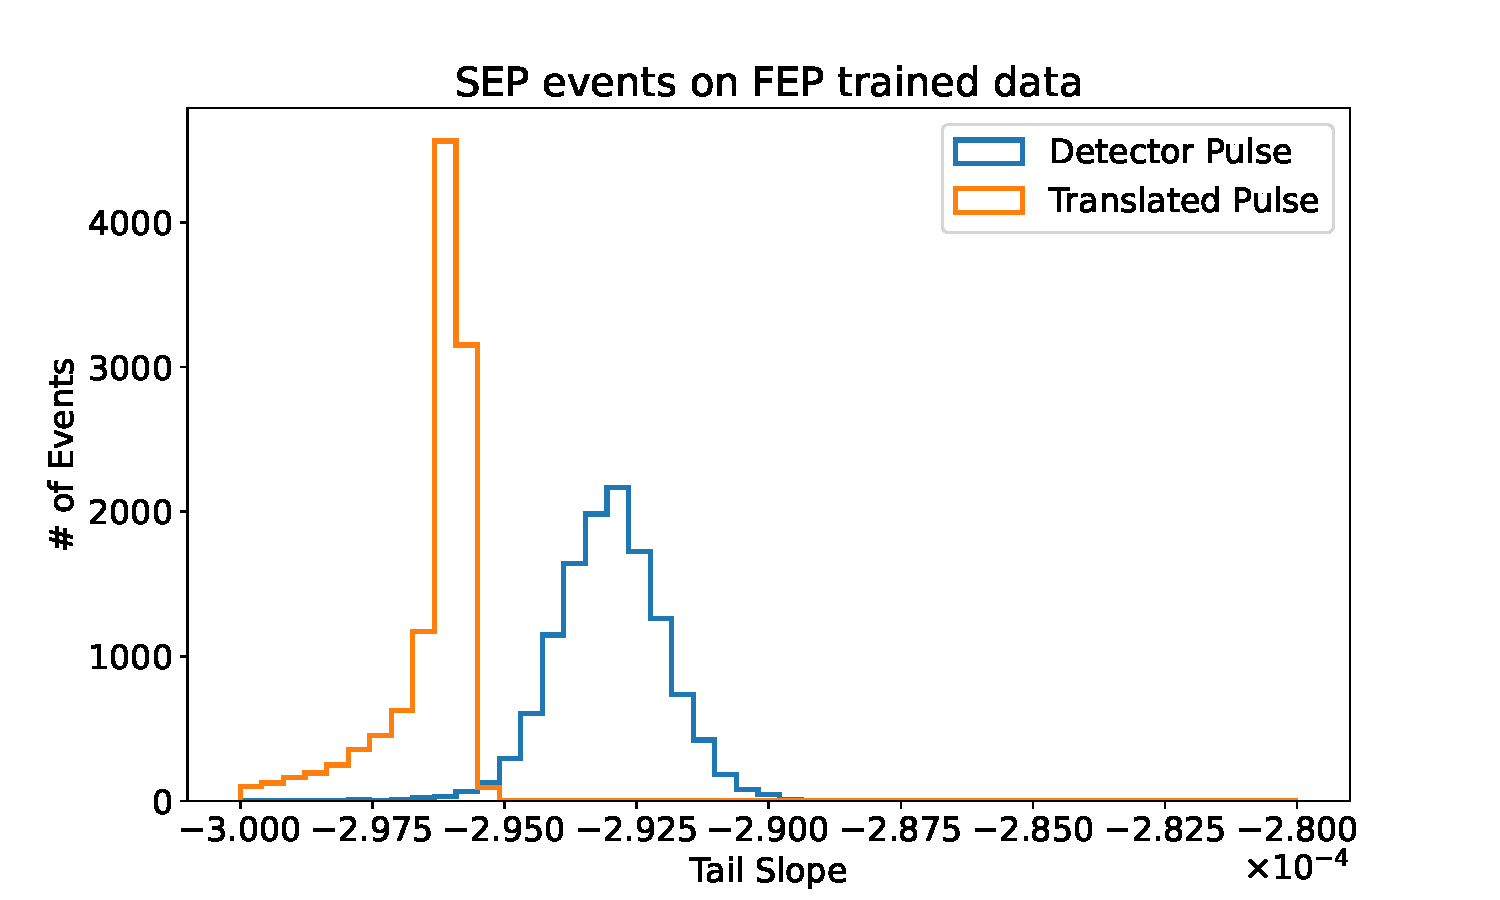
\includegraphics[width=0.99\linewidth,trim={2pc 0pc 2pc 0pc},clip]{ch8/figs/SEP_ts.pdf}
\caption{ Distribution of Tail slope for all three}
\label{ch8:fig:tail_slope_sim}
\end{figure}


Finally, the model reproduces the characteristic RC decay tail observed in real detector data. While the original simulations have zero tail slope, ATN outputs have a mean tail slope within $0.58\%$ of the measured data values, confirming that the network captures this important detector response component without explicit modeling. 

While our primary focus in this paper is on translating simulations to resemble measured data, CPU-Net’s bidirectional nature also makes it a powerful tool for denoising real detector waveforms. By transforming noisy detector signals into cleaner, simulation-like waveforms, CPU-Net can help isolate and identify subtle features in the event topology. This capability could ultimately improve spatial reconstruction and enhance our understanding of particle interactions within the detector.

